\documentclass[a4paper,12pt]{report}
\usepackage[utf8]{inputenc}
\usepackage[T1]{fontenc}
\usepackage[polish]{babel}
\usepackage{graphicx}
\usepackage{geometry}
\usepackage{titlesec}
\usepackage{float}
\usepackage{indentfirst}
\usepackage{tcolorbox}
\usepackage{url}
\usepackage{caption}
\usepackage{listings}
\usepackage[space]{grffile} 
\usepackage{afterpage}


\geometry{margin=1in}

% Ustawienia czcionki Times New Roman
\renewcommand{\rmdefault}{ptm}  % Times New Roman

% Styl tytułów rozdziałów i podrozdziałów
\titleformat{\section}[hang]
  {\bfseries\fontsize{14}{16}\selectfont}  % Tytuł rozdziału w Times New Roman, bold, 14 pt
  {\thesection}{1em}{}
  
\titleformat{\subsection}[hang]
  {\bfseries\fontsize{12}{14}\selectfont}  % Tytuł podrozdziału w Times New Roman, bold, 12 pt
  {\thesubsection}{1em}{}
  \lstset{
    basicstyle=\ttfamily\footnotesize,
    frame=single,
    breaklines=true,
    numbers=none
}

\tcbset{
    myframe/.style={
        colback=white,
        colframe=black,
        coltitle=black,
        sharp corners=all,
        boxrule=0.5pt,
        width=\textwidth,
        arc=3mm,
        left=1mm,
        right=1mm,
        bottom=1mm,
        top=1mm,
    },
}

\begin{document}

\begin{titlepage}
    \centering
    \raggedright{
\includegraphics[width=15.0cm, height=4.0cm]{logoWSIiZ.PNG}}

    \vspace*{1cm}
    \raggedright{{\bfseries\fontsize{16}{18}\selectfont KOLEGIUM INFORMATYKI STOSOWANEJ}\\[1cm]}

    \raggedright{{\fontsize{14}{16}\selectfont \textbf{Kierunek: INFORMATYKA}}\\[0.5cm]
    {\fontsize{14}{16}\selectfont \textbf{Grupa: 3IIZ/2026 L2}}}\\[2cm]

    \begin{center}
        {\fontsize{14}{16}\selectfont \textbf{Wiktor Nicpoń}}\\
        {\fontsize{14}{16}\selectfont Nr albumu studenta: 71343}
    \end{center}
    \begin{center}
    {\bfseries\itshape\fontsize{20}{24}\selectfont Program Sklep}\\[0.5cm]

    {\fontsize{14}{16}\selectfont Pod kierunkiem: mgr inż. Ewa Żesławska}\\[4cm]

    {\bfseries\fontsize{18}{22}\selectfont \textbf{PROJEKT}}\\[5cm]
    {\bfseries\fontsize{14}{16}\selectfont Rzeszów 2026}
    \end{center}
    \vfill
\newcommand\blankpage{%
    \null
    \thispagestyle{empty}%
    \addtocounter{page}{-1}%
    \newpage}
    \afterpage{\blankpage}
\end{titlepage}
\newpage

% --- SPIS TREŚCI ---
\tableofcontents
\newpage

% --- WSTĘP ---
\chapter*{Wstęp}
\addcontentsline{toc}{chapter}{Wstęp}

Celem niniejszego projektu było zaprojektowanie i zaimplementowanie aplikacji konsolowej w języku C\#, służącej do kompleksowej obsługi sklepu odzieżowego. System wspiera dwa kluczowe obszary działalności: perspektywę klienta (zakupy, koszyk) oraz perspektywę sprzedawcy (zarządzanie magazynem, administracja użytkownikami).

Aplikacja kładzie nacisk na ergonomię użytkowania w środowisku tekstowym oraz trwałość danych, realizowaną poprzez autorski system zapisu do plików. Kluczowym wyróżnikiem jest implementacja logiki biznesowej rozróżniającej klientów detalicznych i hurtowych. W procesie implementacji ściśle wykorzystano paradygmaty programowania obiektowego, co pozwoliło na stworzenie modularnej i łatwej w rozbudowie struktury kodu. Dodatkowo system wyposażono w mechanizmy walidacji danych wejściowych, zapewniające integralność informacji oraz stabilność działania aplikacji w przypadku błędów użytkownika.

% --- ROZDZIAŁ 1 ---
\chapter{Wymagania projektu}

\section{Wymagania funkcjonalne}
Wymagania funkcjonalne określają zakres operacji, jakie system musi umożliwiać użytkownikom końcowym. Na ich podstawie zaprojektowano strukturę aplikacji oraz sposób jej działania. Obejmują one zarówno funkcje dostępne dla klientów, jak i operacje administracyjne realizowane przez sprzedawcę. Wymagania te stanowią podstawę do poprawnej realizacji procesów sprzedażowych w systemie.

\subsection{Zarządzanie produktami}
System umożliwia sprzedawcy zarządzanie asortymentem sklepu poprzez dodawanie nowych produktów oraz modyfikację istniejących pozycji. Każdy produkt posiada określone cechy, takie jak nazwa, cena oraz ilość dostępna w magazynie. Wprowadzone zmiany są zapisywane w systemie przechowywania danych, co zapewnia aktualność informacji. Funkcjonalność ta pozwala na bieżącą kontrolę oferty sklepu.

\subsection{Zarządzanie zamówieniami}
Proces zakupowy umożliwia klientowi przeglądanie katalogu produktów oraz dodawanie wybranych pozycji do koszyka. Zawartość koszyka może być modyfikowana przed finalizacją zamówienia. Po zatwierdzeniu koszyka system zapisuje dane zamówienia oraz aktualizuje stany magazynowe. Każde zamówienie jest przypisane do konkretnego użytkownika.

\subsection{Autoryzacja i uwierzytelnianie}
System obsługuje mechanizmy rejestracji oraz logowania użytkowników. Wyróżniono trzy role użytkowników, z których każda posiada inny zakres uprawnień. Sprzedawca ma dostęp do funkcji administracyjnych, natomiast klienci mogą realizować proces zakupowy. Klient hurtowy otrzymuje automatycznie naliczany rabat w wysokości 10\%.

\section{Wymagania niefunkcjonalne}
Wymagania niefunkcjonalne opisują cechy systemu wpływające na jego jakość i komfort użytkowania. Obejmują one aspekty takie jak wydajność, trwałość danych oraz użyteczność interfejsu.

\begin{itemize}
    \item \textbf{Wydajność:} System powinien reagować szybko na działania użytkownika. Zastosowanie plików tekstowych jako mechanizmu przechowywania danych pozwala na sprawne przetwarzanie informacji bez dużego obciążenia systemu.

    \item \textbf{Trwałość danych:} Dane aplikacji są zapisywane w plikach tekstowych w katalogu \texttt{Data}, co umożliwia ich zachowanie pomiędzy kolejnymi uruchomieniami programu. Każda istotna operacja skutkuje aktualizacją odpowiednich plików.

    \item \textbf{Użyteczność:} Interfejs konsolowy został zaprojektowany z myślą o czytelności i prostocie obsługi. Wykorzystano kolory oraz komunikaty tekstowe w celu ułatwienia nawigacji i interpretacji informacji.
\end{itemize}

% --- ROZDZIAŁ 2 ---
\chapter{Opis struktury projektu}

\section{Struktura plików i klas}
Struktura projektu została zaprojektowana w sposób modułowy, co umożliwia czytelne rozdzielenie odpowiedzialności poszczególnych elementów aplikacji. Architektura systemu opiera się na logicznym podziale na warstwy, co ułatwia organizację kodu oraz jego późniejszą rozbudowę. Na rysunku \ref{fig:diagram_klas} przedstawiono diagram klas ilustrujący strukturę projektu oraz zależności pomiędzy kluczowymi elementami systemu.

\begin{figure}[H]
    \centering
    \includegraphics[
        width=\textwidth,
        keepaspectratio
    ]{diagram klas.png}
    \caption{Diagram klas projektu}
    \label{fig:diagram_klas}
\end{figure}

Główne elementy struktury projektu obejmują:
\begin{itemize}
    \item \textbf{Models:} Zawiera klasy reprezentujące podstawowe obiekty systemu, takie jak użytkownik, produkt oraz zamówienie, które odzwierciedlają dane przetwarzane przez aplikację.
    \item \textbf{Repositories:} Odpowiada za obsługę zapisu i odczytu danych z plików tekstowych, pełniących rolę uproszczonej bazy danych.
    \item \textbf{Helpers:} Zawiera funkcje pomocnicze wspierające działanie aplikacji, w tym obsługę koszyka oraz walidację danych wprowadzanych przez użytkownika.
\end{itemize}

% --- ROZDZIAŁ 3 ---
\chapter{Opis techniczny projektu}

\section{Środowisko i konfiguracja}
Aby zapewnić prawidłowe działanie oraz możliwość kompilacji aplikacji "System Zarządzania Sklepem", stacja robocza musi spełniać określone wymagania programowe i sprzętowe. Poniżej przedstawiono szczegółową specyfikację środowiska, w którym projekt został stworzony i przetestowany.

\subsection{Wymagania systemowe i programowe}
Projekt został zrealizowany w oparciu o nowoczesny ekosystem firmy Microsoft, co gwarantuje stabilność i bezpieczeństwo.
\begin{itemize}
    \item \textbf{System operacyjny:} Zalecanym środowiskiem jest \textbf{Microsoft Windows 11}, jednak aplikacja zachowuje pełną kompatybilność również z systemem Windows 10 (wersja 2004 lub nowsza).
    \item \textbf{Środowisko programistyczne (IDE):} Do wytworzenia kodu wykorzystano \textbf{Microsoft Visual Studio 2022} (wersja Community lub Professional).
    \item \textbf{Framework:} Aplikacja bazuje na platformie \textbf{.NET 10.0 LTS} (Long Term Support), co zapewnia długoterminowe wsparcie techniczne oraz dostęp do najnowszych funkcjonalności języka C\#.
    \item \textbf{Szablon projektu:} Wybrano szablon \textbf{"Aplikacja konsoli" (Console Application)}, który jest optymalny dla systemów operujących na interfejsie tekstowym, zapewniając minimalny narzut wydajnościowy.
\end{itemize}

Opisane środowisko programistyczne zapewnia możliwość bezproblemowej kompilacji, uruchamiania oraz dalszego rozwoju aplikacji zarówno w warunkach laboratoryjnych, jak i domowych.

\subsection{Wymagania sprzętowe}
Ze względu na konsolowy charakter aplikacji oraz zastosowanie lekkiej bazy danych opartej na plikach tekstowych, wymagania sprzętowe są minimalne:
\begin{itemize}
    \item \textbf{Procesor:} Jednostka o architekturze x64 lub ARM64 o taktowaniu min. 1 GHz.
    \item \textbf{Pamięć RAM:} Minimum 512 MB dostępnej pamięci operacyjnej (zalecane 4 GB dla komfortowej pracy z Visual Studio).
    \item \textbf{Przestrzeń dyskowa:} Aplikacja wymaga zaledwie ok. \textbf{50 MB} wolnej przestrzeni dyskowej. Wartość ta obejmuje skompilowane pliki wykonywalne (.exe, .dll) oraz katalog \texttt{Data} przechowujący pliki tekstowe bazy danych.
\end{itemize}

\section{Mechanizm przechowywania danych}
Zastosowano autorski mechanizm przechowywania danych oparty na plikach tekstowych (.txt) z separatorem średnikowym. Rozwiązanie to pełni rolę uproszczonej bazy danych i umożliwia trwały zapis informacji pomiędzy kolejnymi uruchomieniami aplikacji.

\begin{itemize}
    \item \textbf{users.txt} – Plik przechowujący dane użytkowników oraz informacje o ich rolach w systemie.
    \item \textbf{products.txt} – Plik zawierający katalog produktów dostępnych w sklepie.
    \item \textbf{orders.txt} – Plik przechowujący historię zrealizowanych transakcji.
\end{itemize}

% --- ROZDZIAŁ 4 ---
\chapter{Harmonogram prac}

\section{Diagram Gantta}
Poniższy wykres prezentuje rozkład prac związanych z realizacją projektu w czasie. Harmonogram obejmuje wszystkie kluczowe etapy tworzenia aplikacji, począwszy od analizy wymagań, poprzez projektowanie oraz implementację systemu, aż po testowanie i przygotowanie dokumentacji końcowej.

Na rysunku \ref{fig:gantt} przedstawiono diagram Gantta ilustrujący kolejność realizacji poszczególnych zadań oraz czas ich trwania. Część etapów była realizowana równolegle, co pozwoliło na efektywne wykorzystanie dostępnego czasu. Takie podejście odzwierciedla rzeczywisty przebieg prac projektowych oraz umożliwiło terminowe zakończenie projektu.

\begin{figure}[H]
    \centering
    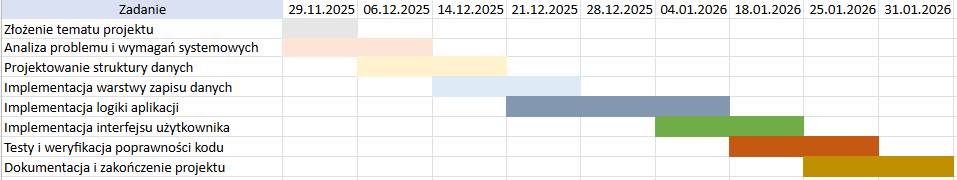
\includegraphics[
        width=\textwidth,
        height=5.5\textheight,
        keepaspectratio
    ]{Gant.png}
    \caption{Diagram Gantta}
    \label{fig:gantt}
\end{figure}

% --- ROZDZIAŁ 5 ---
\chapter{Repozytorium i system kontroli wersji}

W trakcie realizacji projektu wykorzystano system kontroli wersji Git, który umożliwiał bieżące zarządzanie kodem źródłowym oraz śledzenie historii wprowadzanych zmian. Zastosowanie repozytorium pozwalało na systematyczne zapisywanie kolejnych etapów prac, a także ułatwiało testowanie aplikacji oraz eliminację błędów pojawiających się w trakcie implementacji. Kod źródłowy był wersjonowany lokalnie, a następnie publikowany w zdalnym repozytorium.

Repozytorium projektu zostało udostępnione w serwisie GitHub, co umożliwia wgląd w pliki projektu oraz pliku z dokumentacją˛. Podstawowa struktura repozytorium została przedstawiona na rysunku \ref{fig:Repo}. Repozytorium dostępne jest pod adresem:
\url{https://github.com/WiktorNicpon/Programowanie.git}

\begin{figure}[H]
    \centering
    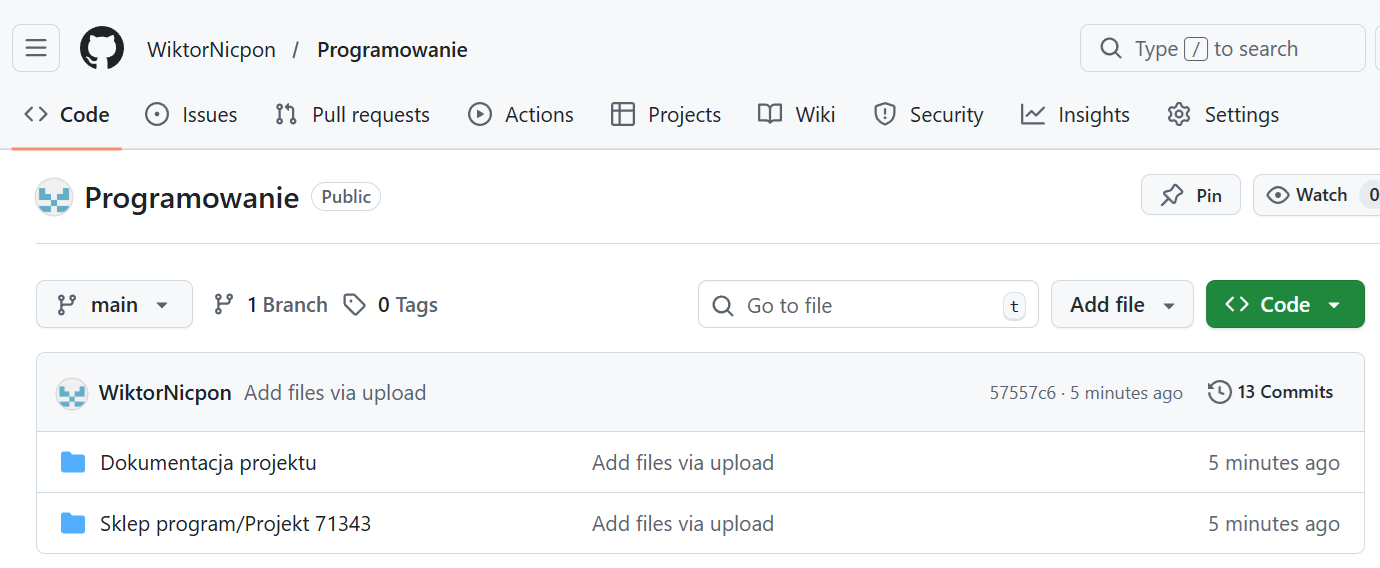
\includegraphics[
        width=\textwidth,
        height=5.5\textheight,
        keepaspectratio
    ]{Repo.png}
    \caption{Struktura repozytorium projektu w serwisie GitHub}
    \label{fig:Repo}
\end{figure}
% --- ROZDZIAŁ 6 ---
\chapter{Prezentacja warstwy użytkowej}

Aplikacja sklepu została zaprojektowana jako rozwiązanie działające w trybie konsolowym. Całość funkcjonalności, obejmująca zarówno mechanizmy przetwarzania danych, jak i sposób prezentacji informacji użytkownikowi, została opracowana w języku C\#. Obsługa programu odbywa się w środowisku tekstowym, bez zastosowania interfejsu graficznego, a komunikacja z systemem realizowana jest wyłącznie za pomocą klawiatury.

W kolejnej części rozdziału zaprezentowano wybrane zrzuty ekranu ilustrujące kluczowe elementy działania aplikacji. Materiały te mają na celu przybliżenie sposobu interakcji użytkownika z systemem oraz przedstawienie organizacji interfejsu konsolowego.

Po uruchomieniu programu wyświetlany jest ekran startowy, który umożliwia wybór trybu pracy aplikacji. Użytkownik może zdecydować, czy chce korzystać z systemu w roli sprzedawcy, czy jako klient, co determinuje dostępny zakres funkcjonalności.

\begin{figure}[H]
    \centering
    \includegraphics[width=0.7\textwidth]{{Menu Główne sklep}.png}
    \caption{Ekran główny aplikacji}
    \label{fig:main}
\end{figure}

\section{Sprzedawca - Zarządzanie systemem}
Logowanie do panelu sprzedawcy wymaga uprawnień administratora (Rysunek \ref{fig:log_seller}).

\begin{figure}[H]
    \centering
    \includegraphics[width=0.7\textwidth]{{logowanie sprzedawcy}.png}
    \caption{Logowanie do panelu sprzedawcy}
    \label{fig:log_seller}
\end{figure}

Sprzedawca po zalogowaniu ma dostęp do kluczowych funkcji zarządczych (Rysunek \ref{fig:panel_seller}).

\begin{figure}[H]
    \centering
    \includegraphics[width=0.7\textwidth]{{panel sprzedawcy}.png}
    \caption{Menu główne sprzedawcy}
    \label{fig:panel_seller}
\end{figure}

Menu sprzedawcy umożliwia dostęp do wszystkich funkcji administracyjnych systemu. Z jego poziomu możliwe jest zarządzanie magazynem, przeglądanie historii zamówień oraz administracja kontami użytkowników.

\subsection{Zarządzanie magazynem}
Sprzedawca może weryfikować stany magazynowe. Poniżej przedstawiono proces dodawania nowego towaru.
Najpierw widoczny jest stan początkowy (Rysunek \ref{fig:stock_start}), następnie dodanie produktu "Kurtka" (Rysunek \ref{fig:add_stock}), a na końcu zaktualizowana lista produktów (Rysunek \ref{fig:stock_end}).

\begin{figure}[H]
    \centering
    \includegraphics[width=0.7\textwidth]{{stan magazynu z widoku sprzedawcy}.png}
    \caption{Stan magazynu przed dostawą}
    \label{fig:stock_start}
\end{figure}

\begin{figure}[H]
    \centering
    \includegraphics[width=0.7\textwidth]{{dodanie nowego produktu do magazynu}.png}
    \caption{Proces dodawania nowego produktu (Kurtka)}
    \label{fig:add_stock}
\end{figure}

\begin{figure}[H]
    \centering
    \includegraphics[width=0.7\textwidth]{{zaktualizowany stan magazynu}.png}
    \caption{Stan magazynu po aktualizacji - widoczna nowa pozycja}
    \label{fig:stock_end}
\end{figure}

Przedstawiony scenariusz ilustruje pełny proces aktualizacji magazynu, począwszy od przeglądu stanu początkowego, aż do potwierdzenia wprowadzenia nowego produktu do systemu.

\subsection{Wyświetlenie historii zamówień}
Widok historii zamówień umożliwia sprzedawcy wgląd w zrealizowane transakcje poszczególnych klientów. Informacje te pozwalają na kontrolę sprzedaży oraz weryfikację poprawności działania systemu zamówień.

\begin{figure}[H]
    \centering
    \includegraphics[width=0.7\textwidth]{{Historia zamówień}.png}
    \caption{Historia zamówień poszczególnych klientów}
    \label{fig:orders_history}
\end{figure}

\subsection{Zarządzanie klientami}
Administrator posiada uprawnienia do usuwania użytkowników. Poniżej zaprezentowano listę klientów przed operacją (Rysunek \ref{fig:client_list_pre}), proces usuwania klienta (Rysunek \ref{fig:client_del}) oraz zaktualizowaną listę (Rysunek \ref{fig:client_list_post}).

\begin{figure}[H]
    \centering
    \includegraphics[width=0.8\textwidth]{{lista klientów}.png}
    \caption{Lista klientów przed usunięciem}
    \label{fig:client_list_pre}
\end{figure}

\begin{figure}[H]
    \centering
    \includegraphics[width=0.8\textwidth]{{usunięcie klienta przez sprzedawce}.png}
    \caption{Usuwanie użytkownika z bazy po adresie email}
    \label{fig:client_del}
\end{figure}

\begin{figure}[H]
    \centering
    \includegraphics[width=0.8\textwidth]{{lista klientów po usunięciu klienta Wiktor}.png}
    \caption{Zaktualizowana lista klientów (brak użytkownika Wiktor)}
    \label{fig:client_list_post}
\end{figure}

Proces usuwania klienta z systemu został zaprojektowany w sposób prosty i jednoznaczny. Po wykonaniu operacji lista użytkowników jest natychmiast aktualizowana, co potwierdza poprawne działanie mechanizmu administracyjnego.

\section{Klient - Scenariusze zakupowe}
Aplikacja obsługuje zarówno klientów detalicznych, jak i hurtowych. W tej części zaprezentowano typowe scenariusze zakupowe realizowane przez użytkowników systemu. Przebieg procesu różni się w zależności od rodzaju konta, co pozwala na zastosowanie odmiennych zasad cenowych.

\subsection{Scenariusz Klienta Detalicznego}
Nowy użytkownik rozpoczyna od rejestracji (Rysunek \ref{fig:reg_detal}). Wybór opcji "n" przy pytaniu o konto hurtowe tworzy standardowe konto detaliczne.

\begin{figure}[H]
    \centering
    \includegraphics[width=0.7\textwidth]{{rejestracja klienta}.png}
    \caption{Rejestracja klienta detalicznego}
    \label{fig:reg_detal}
\end{figure}

Następnie następuje logowanie (Rysunek \ref{fig:login_cl}).

\begin{figure}[H]
    \centering
    \includegraphics[width=0.7\textwidth]{{Logowanie klienta}.png}
    \caption{Logowanie do systemu}
    \label{fig:login_cl}
\end{figure}

Po zalogowaniu klient widzi swój panel (Rysunek \ref{fig:panel_detal}). Brak oznaczeń o zniżkach potwierdza status detaliczny.

\begin{figure}[H]
    \centering
    \includegraphics[width=0.7\textwidth]{{panel klienta detalicznego}.png}
    \caption{Panel klienta detalicznego}
    \label{fig:panel_detal}
\end{figure}

Klient przegląda katalog (Rysunek \ref{fig:catalog}), wybiera produkt i dodaje go do koszyka (Rysunek \ref{fig:buy_detal}). Ceny są standardowe.

\begin{figure}[H]
    \centering
    \includegraphics[width=0.7\textwidth]{{katalog produktów}.png}
    \caption{Katalog produktów}
    \label{fig:catalog}
\end{figure}

\begin{figure}[H]
    \centering
    \includegraphics[width=0.7\textwidth]{{udany zakup detaliczny}.png}
    \caption{Dodawanie produktu do koszyka}
    \label{fig:buy_detal}
\end{figure}

W koszyku widoczne jest podsumowanie bez naliczonego rabatu (Rysunek \ref{fig:cart_detal}).

\begin{figure}[H]
    \centering
    \includegraphics[width=0.7\textwidth]{{koszyk po dodaniu produktu.}.png}
    \caption{Koszyk klienta detalicznego}
    \label{fig:cart_detal}
\end{figure}

\begin{figure}[H]
    \centering
    \includegraphics[width=0.7\textwidth]{{moje dane klienta}.png}
    \caption{Dane klienta detalicznego (dane wyświetlone po zakupie w sklepie)}
    \label{fig:client_data}
\end{figure}

Przedstawiony scenariusz pokazuje standardowy proces zakupowy bez naliczania dodatkowych rabatów. Wszystkie ceny prezentowane są w wartości podstawowej, co jednoznacznie identyfikuje użytkownika jako klienta detalicznego.

\subsection{Scenariusz Klienta Hurtowego}
System rozróżnia klientów biznesowych. Rejestracja konta hurtowego wymaga potwierdzenia opcji (Rysunek \ref{fig:reg_hurt}).

\begin{figure}[H]
    \centering
    \includegraphics[width=0.7\textwidth]{{rejestracja klienta hurtowego}.png}
    \caption{Rejestracja konta hurtowego}
    \label{fig:reg_hurt}
\end{figure}

Panel hurtownika (Rysunek \ref{fig:panel_hurt}) wyraźnie informuje o aktywnej zniżce -10\%.

\begin{figure}[H]
    \centering
    \includegraphics[width=0.7\textwidth]{{panel klienta hurtowego}.png}
    \caption{Panel klienta hurtowego ze zniżką}
    \label{fig:panel_hurt}
\end{figure}

Podczas zakupów system automatycznie przelicza ceny. W koszyku hurtownika (Rysunek \ref{fig:cart_hurt}) cena końcowa jest obniżona i wyróżniona kolorem zielonym.

\begin{figure}[H]
    \centering
    \includegraphics[width=0.7\textwidth]{{koszyk klienta hurtowego po dodaniu produktu}.png}
    \caption{Koszyk z naliczonym rabatem hurtowym}
    \label{fig:cart_hurt}
\end{figure}

Zatwierdzenie koszyka kończy transakcję (Rysunek \ref{fig:order_ok}).

\begin{figure}[H]
    \centering
    \includegraphics[width=0.7\textwidth]{{zatwierdzenie zakupu}.png}
    \caption{Potwierdzenie złożenia zamówienia}
    \label{fig:order_ok}
\end{figure}

\begin{figure}[H]
    \centering
    \includegraphics[width=0.7\textwidth]{{dane klienta hurtowego}.png}
    \caption{Dane klienta hurtowego (dane wyświetlone po zakupie w sklepie)}
    \label{fig:client_data}
\end{figure}

W przypadku klienta hurtowego system automatycznie uwzględnia rabat procentowy podczas obliczania wartości zamówienia. Informacja o obniżonej cenie jest wyraźnie widoczna w interfejsie, co zwiększa przejrzystość procesu zakupowego.

% --- ROZDZIAŁ 7 ---
\chapter{Podsumowanie}

\section{Wnioski z realizacji projektu}
Projekt „System Zarządzania Sklepem” został pomyślnie zrealizowany zgodnie z założonymi wymaganiami funkcjonalnymi i niefunkcjonalnymi. Opracowana aplikacja konsolowa umożliwia kompleksową obsługę podstawowych procesów związanych z funkcjonowaniem sklepu odzieżowego. System w poprawny sposób realizuje kluczowe operacje, takie jak zarządzanie asortymentem, obsługa zamówień oraz administracja użytkownikami.

Aplikacja spełnia wszystkie założenia funkcjonalne, poprawnie obsługując:
\begin{itemize}
    \item zarządzanie bazą towarową (operacje typu CRUD) przez sprzedawcę,
    \item administrację kontami użytkowników, w tym usuwanie klientów z systemu,
    \item procesy sprzedażowe z uwzględnieniem różnych ról użytkowników (klient detaliczny oraz hurtowy).
\end{itemize}

Przeprowadzone testy potwierdziły poprawność działania systemu oraz prawidłową aktualizację danych zapisywanych w plikach tekstowych. Zastosowane rozwiązania zapewniają stabilność działania aplikacji oraz spójność przechowywanych informacji.

\section{Plany rozbudowy}
W przyszłości planowana jest dalsza rozbudowa aplikacji w celu zwiększenia jej funkcjonalności oraz komfortu użytkowania. Jednym z kierunków rozwoju jest wdrożenie graficznego interfejsu użytkownika w technologii WPF, co pozwoli na bardziej intuicyjną obsługę systemu. Dodatkowo rozważana jest migracja mechanizmu przechowywania danych z plików tekstowych do relacyjnej bazy danych SQL, co umożliwi lepszą skalowalność oraz integrację z innymi systemami.

\chapter*{Bibliografia}
\addcontentsline{toc}{chapter}{Bibliografia}

\begin{enumerate}
    \item Dokumentacja Microsoft .NET, \url{https://learn.microsoft.com/pl-pl/dotnet/}.
    \item Matulewski J., C#: lekcje programowania: praktyczna nauka programowania dla platform .NET i .NET Core, Helion, Gliwice 2021
    \item  Kurs edukacyjny wideo dotyczący podstaw języka C\#, dostęp online:
\url{https://youtu.be/zP6BAsUlD_A}.
\end{enumerate}

\end{document}